
% --- INICIO DEL CONTENIDO ---

\section{Contexto y Motivación del Problema}
Los incendios forestales son un problema recurrente a nivel mundial, con graves impactos sobre la flora, fauna e infraestructura. Debido a la influencia humana en su origen y a la complejidad de su control y combate, es fundamental desarrollar enfoques preventivos que permitan reducir sus efectos y optimizar los recursos en la preparación frente a ellos. En Chile, su alta frecuencia motiva la búsqueda de modelos que apoyen la predicción, prevención y preparación frente a estos desastres.

Los datos fueron recolectados de incendios forestales en el Parque de Montesinho, Portugal, buscando un modelo predictivo específico para esta zona enfocado en el tamaño del incendio (área total). Esto no sólo permite un nivel de predicción sobre la existencia de incendios, sino que también la modelación de su potencial tamaño, lo que permite preparativos especiales en base a su predicción  y una mejor optimización de recursos. Pero también implica que errores sistematicos (subestimar incendios grandes) tienen consecuencias reales sobre personas y ecosistemas, lo que es una consideración ética a tener en cuenta.

Los datos provienen del conjunto \textit{Forest Fires} del repositorio público UCI Machine Learning Repository. Cada fila representa el reporte de un lugar específico (coordenadas espaciales X, Y) en un mes y día de la semana particular, junto con sus condiciones meteorológicas e índices de riesgo ese día. Además, la variable respuesta corresponde a la variable \texttt{area}, que es el área quemada del parque (en hectáreas).Se puede ver un pequeño resumen del dataset en Tabla~\ref{tab:variables}. El dataset tiene un total de 517 entradas, y aparte no tiene datos faltantes.

\begin{lstlisting}[caption={Tamaño muestral y datos faltantes}, label={lst:summary}]
    nrow(datos_limpios[0])
    [1] 517
    sum(is.na(datos_limpios))
    [1] 0
\end{lstlisting}

\begin{table}[h!]
\caption{Ficha de variables del conjunto de datos Forest Fires}
\label{tab:variables}
\footnotesize                          
\renewcommand{\arraystretch}{1.25}     
    \begin{tabularx}{\textwidth}{l l l X l l}
    \hline
    \textbf{Variable} & \textbf{Rol} & \textbf{Tipo} & \textbf{Descripción} & \textbf{Unidades} & \textbf{Vals. nulos} \\
    \hline
    X     & Covariable & Entero     & Coordenada espacial eje X en el mapa del parque (1--9)   &        & no \\
    Y     & Covariable & Entero     & Coordenada espacial eje Y en el mapa del parque (1--9)   &        & no \\
    month & Covariable & Categórica & Mes del año: \texttt{jan} hasta \texttt{dec}              &        & no \\
    day   & Covariable & Categórica & Día de la semana: \texttt{mon} hasta \texttt{sun}         &        & no \\
    FFMC  & Covariable & Continuo   & Código de Humedad de los Combustibles Finos, estima el contenido de humedad de materiales combustibles pequeños en superficie: 18.7--96.2                   &        & no \\
    DMC   & Covariable & Continuo   & Código de Humedad del Mantillo, estima el contenido de humedad de materiales combustibles de tamaño medio: 1.1--291.3                    &        & no \\
    DC    & Covariable & Continuo   & Código de Sequía, estima el contenido de humedad de materiales combustibles de tamaño grueso: 7.9--860.6                     &        & no \\
    ISI   & Covariable & Continuo   & Índice de Propagación Inicial, estima la velocidad de propagación de un incendio en terrenos llanos: 0.0--56.1                     &        & no \\
    temp  & Covariable & Continuo   & Temperatura: 2.2--33.3                                    & °C     & no \\
    RH    & Covariable & Entero     & Humedad relativa: 15--100                                 & \%     & no \\
    wind  & Covariable & Continuo   & Velocidad del viento: 0.4--9.4                            & km/h   & no \\
    rain  & Covariable & Continuo   & Lluvia exterior: 0.0--6.4                                 & mm/m\textsuperscript{2} & no \\
    area  & Respuesta  & Continuo   & Superficie forestal quemada: 0.0--1090.8                  & héctareas     & no \\
    \hline
    \end{tabularx}
\\[4pt]  % pequeño espacio
{\footnotesize \textit{Nota.} Las definiciones de los índices FFMC, DMC, DC e ISI
fueron tomadas de Cortez \& Morais (2007, p.~3).}
\end{table}

\section{Objetivo del Análisis}

El objetivo de este trabajo es \textbf{predictivo} y busca responder a la siguiente pregunta de investigación:

\begin{tcolorbox}[colback=gray!10!white,colframe=black,center,width=0.8\textwidth]
    \textbf{¿Qué variables meteorológicas e índices FWI permiten predecir el área quemada en incendios del Parque de Montesinho?}
\end{tcolorbox}

Esto será medido en base a una división de datos, utilizando una división 80/20 para entrenamiento y prueba.

%Declaración explícita de si el objetivo es \textbf{predictivo} o \textbf{descriptivo}. \textit{Ejemplo:} El objetivo principal de este trabajo es predictivo. Buscamos ajustar un modelo de regresión lineal múltiple capaz de estimar la extensión del área quemada dada la información meteorológica, evaluando su desempeño en predicción. Alternativamente, si es descriptivo: Buscamos entender la relación estructural e inferir el efecto del viento y la temperatura sobre la magnitud del incendio, controlando por la humedad.

\section{Limpieza, Preparación de Datos y Análisis Exploratorio}
\subsection{Tratamiento de Datos}

No hay datos faltantes. Se codificó las variables categóricas \texttt{day} y \texttt{month} como variables dummies. Las variables categóricas \texttt{month} y \texttt{day} serán incorporadas mediante variables indicadoras (\textit{dummy variables}), utilizando categorías de referencia para evitar colinealidad perfecta. Fuera de eso, no se puede asumir que este fue el orden en que se tomaron los datos porque no se mencionan fechas de observación. Dado que no existe una secuencia temporal explícita de observaciones, no se espera una estructura temporal fuerte en los residuos. Esto será evaluado posteriormente mediante diagnósticos del modelo.

\begin{figure}[h]
    \centering
    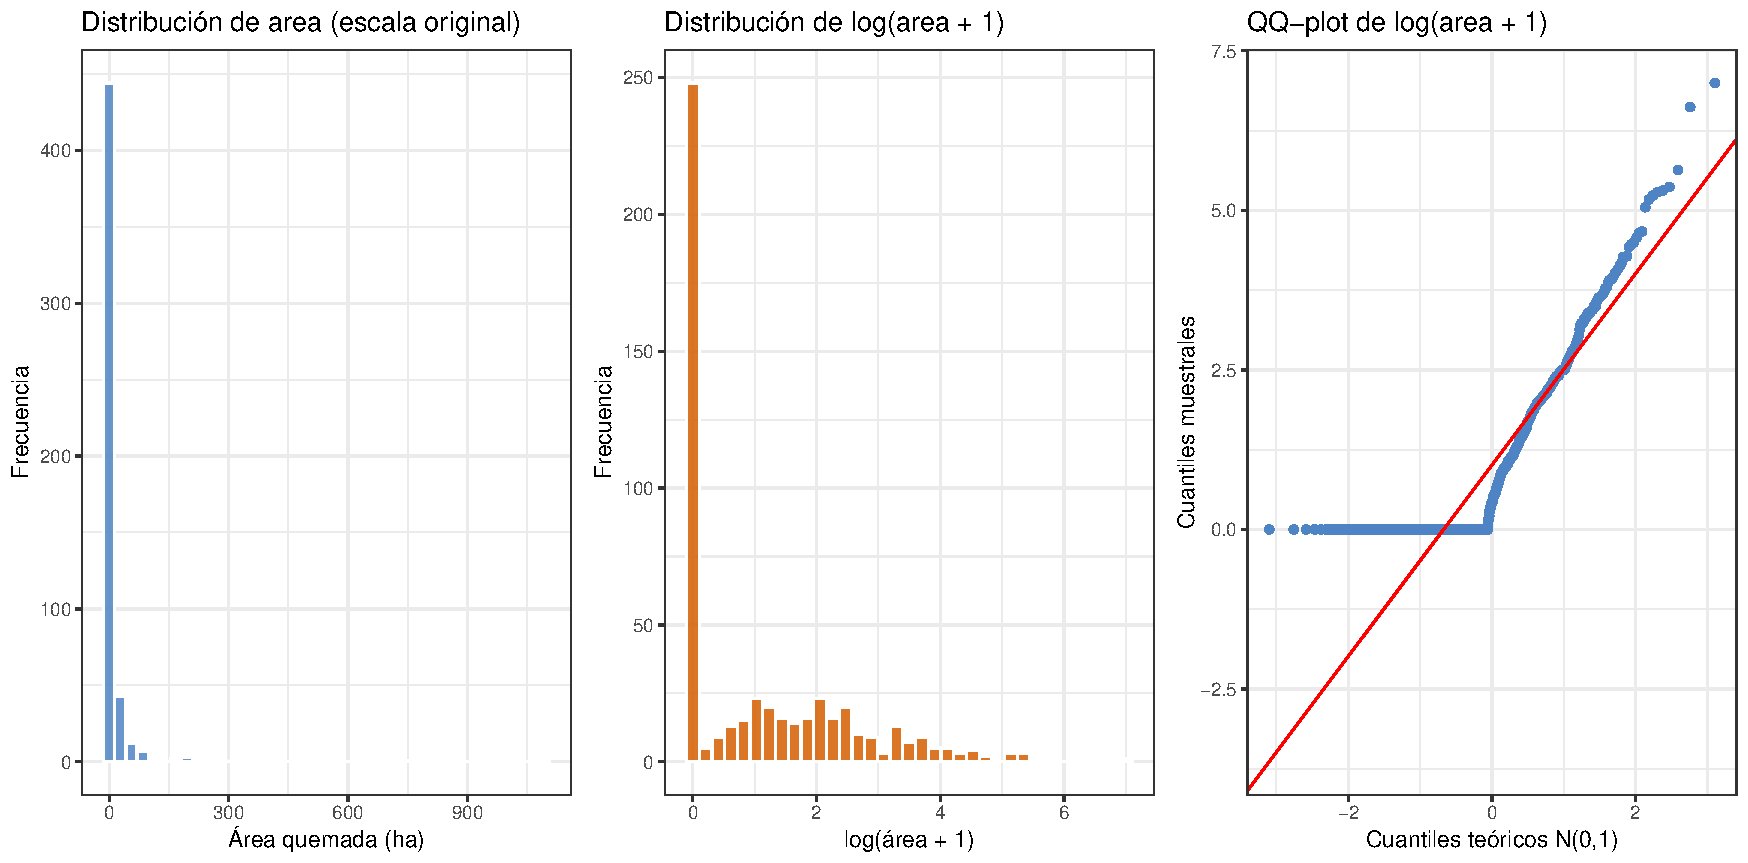
\includegraphics[width=0.9\textwidth]{img/EDA-distribución de la variable de respuesta.pdf}
    \caption{Distribución de la variable de respuesta, original, transformación y QQ-plot}
    \label{img:eda1}
\end{figure}

Hacemos una transformación logaritmica de la respuesta \texttt{area} debido a que tiene una distribución fuertemente asimétrica a la derecha, o sea, la masa de los datos se concentra a la izquierda pero tiene una gran cola hacia la derecha. Lo cual es esperable, la frecuencia de incendios de area pequeña o inexistente \texttt{area}$\:\approx0.0$ es muy grande comparado con la poca frecuencia de incendios de gran envergadura que representan la cola a la derecha de la distribución de la respuesta. Entonces se hace la transformación,
\vspace{8mm}
\begin{lstlisting}[caption={Transformación Logaritmica de Variable Repuesta}, label={lst:log_area}]
    datos_limpios$log_area <- log(datos_limpios$area + 1)
\end{lstlisting}
Se considera el $+1$ en el argumento del logaritmo para que sea exactamente $0$ cuando el \texttt{area} sea $0$. Esto permite estabilizar la varianza y aproximar la distribucion condicional a una normal.

\subsection{Análisis Exploratorio de Datos (EDA)}
%Gráficos bivariados, matrices de correlación y visualización de la distribución de la respuesta.

También de R obtuvimos que la proporción de observaciones con \texttt{area} $ = 0: 47.8\%$ lo cual es otra razón para hacer la transformación logarítmica de la respuesta.
\begin{figure}[h]
    \centering
    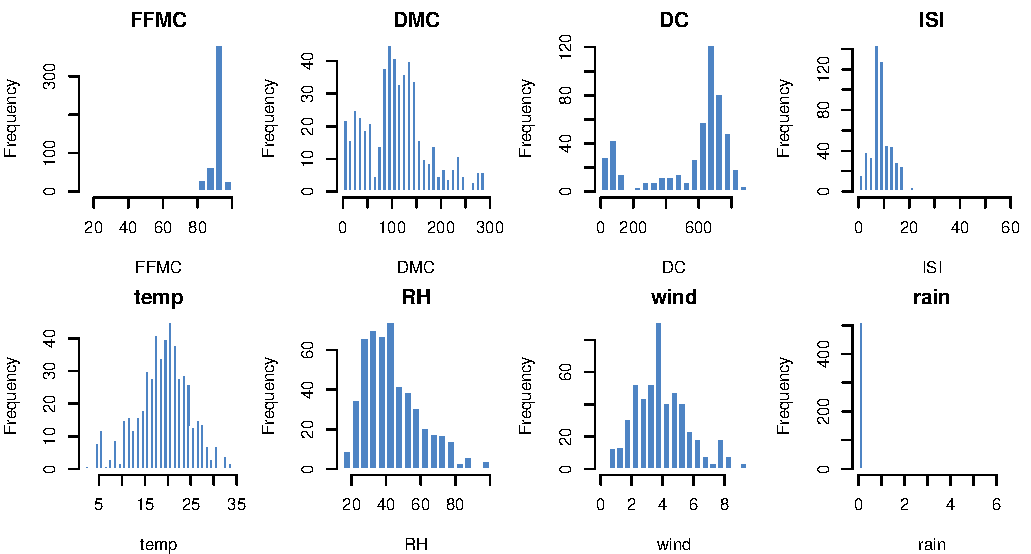
\includegraphics[width=0.8\linewidth]{img/EDA-distribución de las variables numéricas.pdf}
    \caption{Distribución de las variables numéricas}
    \label{img:eda2}
\end{figure}

Observamos en la Imagen~\ref{img:eda2} que las variables de temperatura (\texttt{temp} y \texttt{wind} son más o menos simétricas) las demas son no simétricas o poseen valores extremos que luego se manifestaran como punto de alto leverage. 

\noindent
{\footnotesize \textit{Nota.} De la distribución de la frecuencia de la lluvia (Imagen ~\ref{img:eda2}), vemos que es muy probable que no hará aportes significativos al modelo, pues es una columna casi constante, por lo que habrá problemas con la varianza de su coeficiente asociado.$\textbf{Var}(\beta_j\mid~X)=\frac{\sigma^2}{S_{jj}(1-R_j^2)}$, lo que quiere decir que con los datos que hay no es posible estimar su efecto con precisión. La cantidad de datos mayores a 0 son 8.} 

\begin{figure}[h]
    \centering
    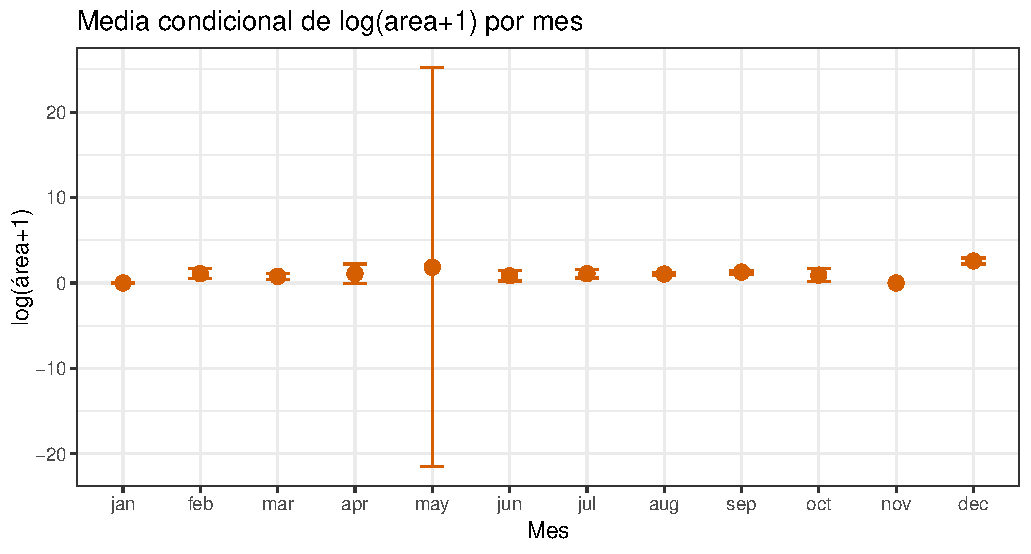
\includegraphics[width=0.5\linewidth]{img/EDA-media condicional del log_area por mes.pdf}
    \caption{Media condicional por mes}
    \label{fig:EDA media cond por mes}
\end{figure}

\begin{table}[h!]
\centering
\footnotesize
\caption{Resumen por mes}
\label{tab:resumen_meses}
\renewcommand{\arraystretch}{1.1}
\setlength{\tabcolsep}{5pt}
    \begin{tabular}{l c c c c c c c c c c c c}
    \hline
    \textbf{Mes}                 & jan & feb  & mar  & apr & may & jun  & jul  & aug  & sep  & oct  & nov & dec \\
    \hline
    \textbf{Cantidad Incendios}  & 2   & 20   & 54   & 9   & 2   & 17   & 32   & 184  & 172  & 15   & 1   & 9   \\
    \textbf{Media}               & 0   & 1.09 & 0.77 & 1.09 & 1.84 & 0.84 & 1.08 & 1.05 & 1.27 & 0.92 & 0   & 2.57 \\
    \hline
    \end{tabular}
\end{table}

\vspace{5em}
Del gráfico de la Imagen~\ref{fig:EDA media cond por mes} y de la salida de R (Tabla ~\ref{tab:resumen_meses}) vemos que las medias condicionales difieren entre meses  por lo que si no agregamos las variables mensuales como \textit{dummies} al modelo este quedará mal especificado y habrá un error asociado a una variable no considerada por lo que podríamos ver algún patron en los residuos que indique que hay estructura sin capturar en el modelo si no las consideramos.

\noindent
\begin{minipage}[t]{0.40\textwidth}
    \vspace{0pt}
    Esta matriz nos dará indicios de colinealidad entre predictores. Se observa que las parejas con mayor correlación en valor absoluto superior a $0.5$ corresponden a variables del sistema FWI y a variables meteorológicas, lo que sugiere una posible dependencia lineal entre ambos grupos. En particular, el índice DMC y el DC comparten un comportamiento conjunto relacionado con la humedad acumulada, mientras que FFMC e ISI están vinculados a la inflamabilidad superficial. La correlación negativa entre temperatura y humedad relativa es esperable desde un punto de vista físico. 
\end{minipage}
\hfill
\begin{minipage}[t]{0.45\textwidth}
    \vspace{5pt}
    \centering
    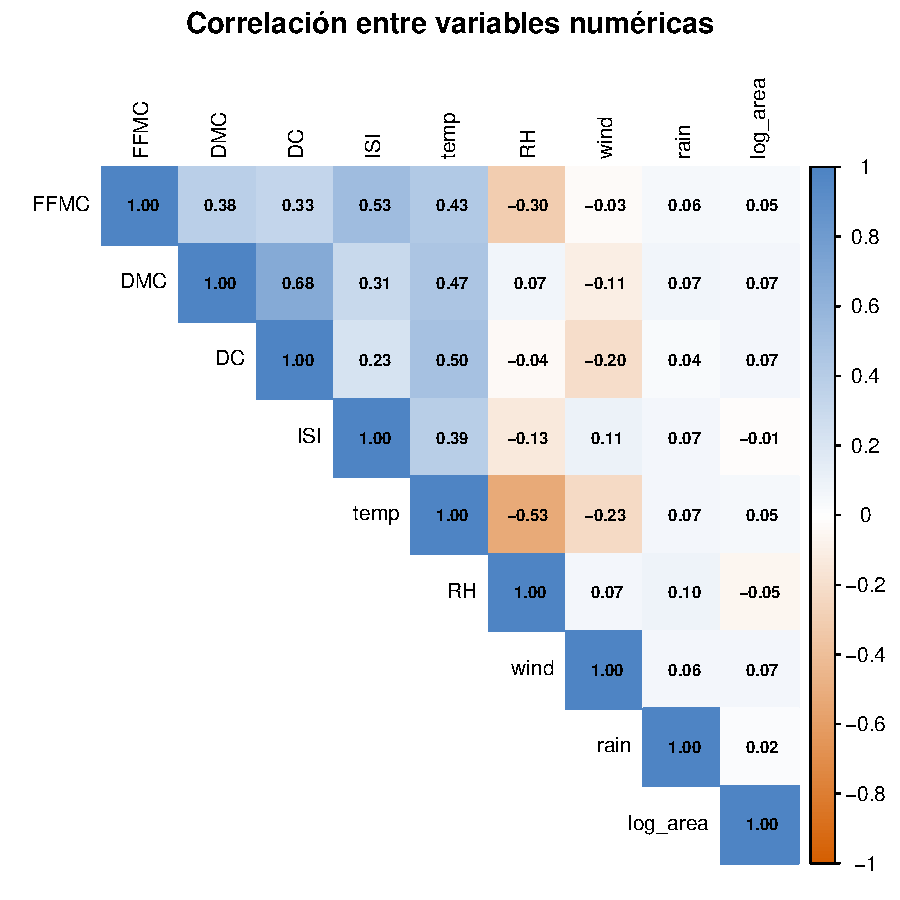
\includegraphics[width=\linewidth]{img/EDA - matriz de correlacion entre predictores.pdf}
    \captionof{figure}{Distribución espacial de incendios}
    \label{fig:distrib_esp_incendios}
\end{minipage}

\noindent
\begin{minipage}[t]{0.42\textwidth}
    \vspace{0pt}
    Las correlaciones más relevantes entre predictores: DMC - DC:   r =  0.682, FFMC - ISI: r =  0.532, temp - RH:  r = -0.527 . La Imagen 5 nos puede ayudar a entender si hay autocorrelación por la estructura espacial, debido a que sectores adyacentes podrían compartir características comunes. Esto lo podremos confirmar posteriormente evaluando si $\text{Cov}(\varepsilon_i, \varepsilon_j) \neq 0$ para $i,j$ adyacentes.
\end{minipage}
\hfill
\begin{minipage}[t]{0.4\textwidth}
    \vspace{5pt}
    \centering
    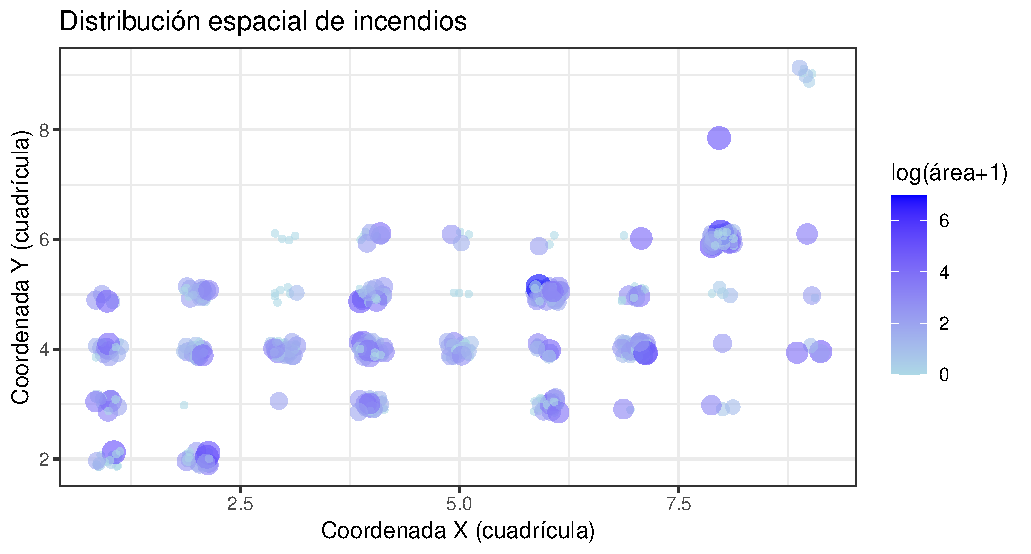
\includegraphics[width=\linewidth]{img/EDA - distribucion espacial de incendios.pdf}
    \captionof{figure}{Distribución espacial de incendios}
    \label{fig:distrib_esp_incendios}
\end{minipage}

\vspace{0.5cm}

\section{Modelos Lineales Candidatos}

El objetivo principal es construir modelos de regresión lineal para estimar el área quemada en incendios forestales del Parque Natural de Montesinho. Para ello, se trabajará sobre la variable respuesta transformada, $\log(\texttt{area} + 1)$. La transformación logarítmica busca una reducción de la fuerte asimetría observada en la variable original y estabilizar la varianza de los residuos.

Todos los modelos considerados asumen la estructura general:
\begin{center}
    $
    \bm{Y} = \bm{X}\bm{\beta} + \bm{\varepsilon},
    \qquad
    \mathbb{E}(\bm{\varepsilon}|\bm{X}) = \bm{0},
    \qquad
    \textbf{Var}(\bm{\varepsilon}|\bm{X}) = \sigma^2 \bm{I}
    $
\end{center}

donde $\bm{Y}$ corresponde al vector de respuestas observadas, $\bm{X}$ a la matriz de diseño, $\bm{\beta}$ al vector de parámetros desconocidos y $\bm{\varepsilon}$ al vector de errores aleatorios.

\vspace{0.3cm}

\begin{itemize}
    \item{Modelo 0: Modelo nulo}
        \begin{center}
            $\log(\texttt{area}+1)=\beta_0+\varepsilon$
        \end{center}

    \item{Modelo 1: Índices FWI}
        \begin{center}
           $\log(\texttt{area}+1)=
            \beta_0+
            \beta_1 FFMC+
            \beta_2 DMC+
            \beta_3 DC+
            \beta_4 ISI+
            \varepsilon
            $
        \end{center}
        
    \item{Modelo 2: Variables meteorológicas}
        \begin{center}
           $\log(\texttt{area}+1)=
            \beta_0+
            \beta_1 temp+
            \beta_2 RH+
            \beta_3 wind+
            \varepsilon
            $
        \end{center}
    
    \item{Modelo 3: Modelo completo numérico}
        \begin{center}
            $\log(\texttt{area}+1)=
            \beta_0+
            \beta_1 FFMC+
            \beta_2 DMC+
            \beta_3 DC+
            \beta_4 ISI+
            \beta_5 temp+
            \beta_6 RH+
            \beta_7 wind+
            \beta_8 rain+
            \varepsilon
            $
        \end{center}
    
    \item{Modelo 4: Incorporación de efectos temporales}
    \begin{center}
        $\log(\texttt{area}+1)=
        \beta_0+
        \beta_1 FFMC+
        \beta_2 DMC+
        \beta_3 DC+
        \beta_4 ISI+
        \beta_5 temp+
        \beta_6 RH+
        \beta_7 wind+
        \texttt{month}+
        \varepsilon
        $
    \end{center}
\end{itemize}

Como referencia inicial, se considerará un modelo con sólo intercepto, el cual servirá como base para evaluar el aporte explicativo de los distintos predictores mediante pruebas globales F.

Posteriormente, se propondrán distintos modelos según el tipo de información incorporada. En primer lugar, se ajustará un modelo utilizando únicamente los índices del sistema canadiense de peligro de incendios (FWI), con el objetivo de evaluar si estos índices poseen capacidad predictiva suficiente sobre el área quemada, considerando que resumen condiciones de inflamabilidad y propagación del fuego.

Luego, se considerará un modelo basado exclusivamente en variables meteorológicas directamente observables, incluyendo temperatura, humedad relativa y viento. Inicialmente se excluirá la variable \texttt{rain}, debido a que presenta una alta proporción de observaciones iguales a cero, lo que podría limitar su aporte al modelo.

Además, se ajustará un modelo completo incorporando todos los predictores numéricos disponibles. Este modelo servirá como punto de partida para realizar análisis de colinealidad y selección de variables. En particular, se evaluará el Factor de Inflación de Varianza (VIF), debido a la posible dependencia lineal entre índices FWI y variables meteorológicas.

Finalmente, se incorporarán variables temporales correspondientes al mes de observación mediante variables dummy, buscando capturar posibles patrones estacionales en la ocurrencia y magnitud de los incendios forestales.

Los modelos candidatos serán comparados utilizando criterios de ajuste e inferencia, tales como $R^2_{aj}$, AIC, suma de cuadrados del error y pruebas F para modelos anidados. Adicionalmente, se utilizará selección automática de variables mediante el algoritmo \text{step()}.

Debido al enfoque predictivo del trabajo, los modelos serán evaluados mediante una división entrenamiento/prueba, utilizando métricas como RMSE y MAE para comparar su desempeño fuera de muestra.

\section{Ajuste e Inferencia}
Interpretar coeficientes clave utilizando salidas de software estadístico. 
Uso de pruebas globales $F$, pruebas $t$ individuales y comparación de modelos anidados vía ANOVA. Reportar el $R^2$ ajustado.

A continuación, un ejemplo de cómo insertar código en R usando nuestra configuración:

\begin{lstlisting}[caption={Ajuste del modelo inicial en R}, label={lst:modelo1}]
# Carga de datos y transformacion
datos <- read.csv("forestfires.csv")
datos$log_area <- log(datos$area + 1)

# Ajuste del Modelo 1 (MCO)
modelo_1 <- lm(log_area ~ temp + RH + wind + rain, data = datos)
summary(modelo_1)

# Tabla ANOVA
anova(modelo_1)
\end{lstlisting}

\section{Diagnóstico del Modelo}
Esta sección es crucial según las clases. Debes reportar:
\begin{itemize}
    \item \textbf{Linealidad y Varianza constante:} Gráfico de residuos versus valores ajustados (Test de Breusch-Pagan).
    \item \textbf{Normalidad de residuos:} Q-Q plot y Test de Shapiro-Wilk (importante si haces inferencia con muestra finita).
    \item \textbf{Colinealidad:} Revisión del Factor de Inflación de Varianza (VIF). ¿Es la geometría de $\bm{X}$ adecuada?
    \item \textbf{Observaciones influyentes:} Distancia de Cook y DFBETAS. Justificar si se excluye algún caso extremo y reportar sensibilidad.
\end{itemize}

\section{Dificultades esperadas}
Entre las principales dificultades esperadas se encuentran:

\begin{itemize}
    \item Fuerte asimetría de la variable respuesta.
    \item Alta presencia de observaciones con área igual a cero.
    \item Posibles observaciones influyentes.
    \item Heterocedasticidad.
    \item Potencial colinealidad entre índices FWI y variables meteorológicas.
\end{itemize}
Estas dificultades deben ser consideradas en el análisis posterior de los modelos, para evitar sesgos a la hora de analizar resultados. 

\section{Conclusiones y Recomendaciones}
Preliminarmente, el conjunto de datos parece adecuado para desarrollar modelos de regresión lineal con fines predictivos. Sin embargo, la fuerte asimetría de la variable respuesta y la alta frecuencia de valores nulos seguramente harán que los diagnósticos y transformaciones sean fundamentales para obtener modelos estadísticamente adecuados.

Cierre conectando las matemáticas con el criterio aplicado. Responder la pregunta inicial: ¿Logramos predecir el área? ¿Qué variables resultaron significativas? Finalmente, proponer una recomendación aplicada basada en la evidencia (por ejemplo, alertas tempranas cuando la temperatura supera cierto umbral y el viento es alto).


